\begin{frame}{Evaluation: Generated Profiles}
  \begin{figure}
    \centering
    \begin{subfigure}[t]{0.48\textwidth}
      \centering
      \caption{Augmented Reality (AR)}
      \label{fig:ar-profile}
      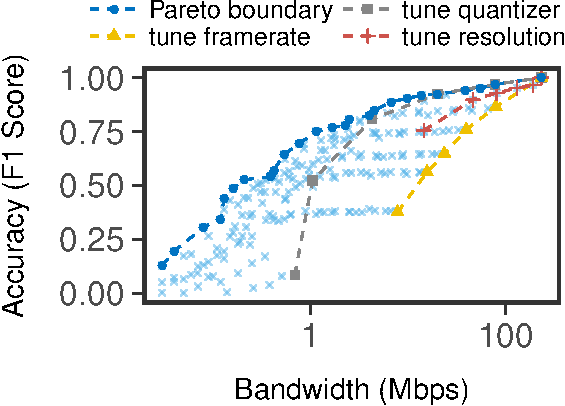
\includegraphics[width=\textwidth]{figures/profile-darknet.pdf}
    \end{subfigure}
    \hfill
    \begin{subfigure}[t]{0.48\textwidth}
      \centering
      \caption{Pedestrian Detection (PD)}
      \label{fig:pd-profile}
      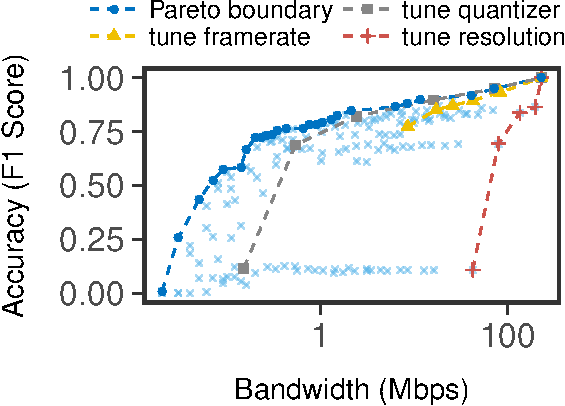
\includegraphics[width=\textwidth]{figures/profile-mot.pdf}
    \end{subfigure}
  \end{figure}

  \begin{itemize}
    \footnotesize
    \visible<2->{
    \item Optimal strategy is achieved with multiple dimensions; tuning one
      dimension leads to suboptimal performance.
    }
    \visible<3->{
    \item For the same application, different dimensions have different impact.
    }
    \visible<4->{\item For different applications, the same dimension has different
      impact.
    }
  \end{itemize}
\end{frame}

\begin{frame}{Evaluation: Generated Profiles (Top-K)}
  \begin{columns}
    \begin{column}{0.45\textwidth}
      \begin{figure}
        \centering
        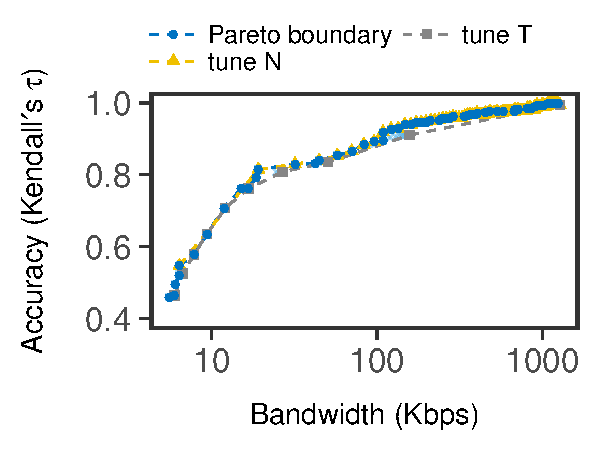
\includegraphics[width=\textwidth]{figures/profile-topk.pdf}
      \end{figure}
    \end{column}
    \begin{column}{0.55\textwidth}
      \begin{itemize}
        \visible<2->{
        \item The effect of each dimension is not significantly different.
        }
        \visible<3->{
        \item The profile offers quantified effects of degradation.
        }
      \end{itemize}
    \end{column}
  \end{columns}
\end{frame}

%%% Local Variables:
%%% mode: latex
%%% TeX-master: "../talk"
%%% TeX-engine: xetex
%%% End:
